\subsection*{Social Media Storage Estimate:}
Social media sites seldom reveals the amount of data they store or ingest on daily basis. Also the ever growing social media makes it hard to estimate their storage capacity. I present few methods in the following section to estimate social media storage.

\Paragraph{1. Storage space estimate from media units:}
This method works for all the social media sites metioned in Table \ref{table:media_units} where the approximate storage space required by media unit is known.

\paragraph{Youtube:}
Lets take an example of Youtube video data. From the Table  \ref{table:media_units} we find by year 2017 users upload 720,000 hours of video in Youtube. First, assuming the fact that Youtube pretty much stores almost
video in 1080p and it stores video in multiple resolution such as 240p, 360p, 720p, 1080p and format e.g. Webm, flv, mp4, 3gp, mp3. We can determine the amount of storage space needed for a 1 minute video \cite{youtube_stats}.

\begin{equation}
\begin{split}
  &27.71 \text{ MB (Webm)} + 17.00 \text{ MB (flv)} + 554.43 \text{ KB (3gp)} \\
  &+ 45.80 \text{ MB (mp4)} + 2.81 \text{ MB (mp3)}\\
  &= 93.8614355 \text{ MB}\\
  \end{split}
\end{equation}
 From the above we find that $720,000 \times 60 \times 93.8614355 \approx 4.055$ petabytes (PB)  of storage space is required by Youtube everyday. We can also calculate the total amount of storage space ingested during the period of 2013 to 2017 from Table \ref{table:media_units} by utilizing area under the curve method with interpolation. The above method reckons 3096.17 PB or 3.096 exabytes (EB) of storage. Considering videos before 2013 and new 4K video which takes more space it can be easily assumed that Youtube use 10-15 EB storage space.

\paragraph{Twitter:}
Similar to the method above we can find the space required to store a tweet. A tweet is stored in Twitter as UTF-8 format. This takes 140 characters tweets atmost 560 bytes of space. However the metadata attached with a tweet is much more than the tweet itself. I personally did a random sample experiment of 100K tweets stord in our databases to find the average storage space for tweet json object obtained from streaming api. I find one json tweet object takes 3247 bytes of space in average.
682 million tweets per day will require around 2.2145 terabytes of data per day. Using the interpolation method for area under the curve we can find that Twitter use 3.13 petabyte of space for storing the tweet alone. It is also worth noting that 42\% of tweets contains images \cite{tweets_images}. If we assume the average image size be 100 KB then we will see $(100 * 1024)/3247 * 42 \% \approx 13.2$ times increase in storage space requirement.

\begin{figure}[t]
	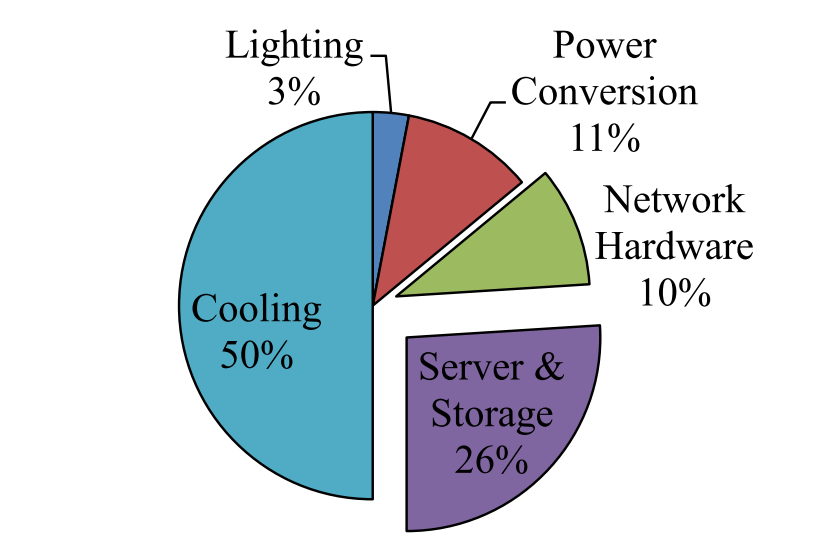
\includegraphics[width=0.7\linewidth ]{fig/energy_usage.png}
    \vspace{-2mm}
    \caption{A typical breakdown of energy usage among components in data center \cite{info2007top}.}
\end{figure}

\Paragraph{2. Storage space estimate from data center power usage:}
This section presents an approximate method to estimate space capacity of large social media companies like Facebook and Google.
A typical breakdown of energy consumption by data center given in Figure \ref{fig:energy_usage}.
The largest energy consuming component is cooling infrastructure with 50\% of total energy. Rest of the energy is used by power conversion, lighting, network and server components \cite{info2007top, dayarathna2016data}. Facebook data centers use efficient data center architecture and hardware tweaks  saves
8-12\% of energy spent in cooling, 13-25\% in power conversion, 10\% in motherboard \cite{frachtenberg2011high}. That implies atmost 11\%  more efficient than typical data centers. Hence, it can be claimed that Facebook servers use 37-38\% of energy. Considering Facebook's 138 MW Altoona data center equipped with 200 Watts servers each with $6\times4$ TB of HDD as used in their experiment for \cite{frachtenberg2011high}. Assuming the datacenter is running at peak energy $(138 \times 0.37 \times 24)/ 200 = 6127200$  TB $= 6.1272$ exabytes (EB).
Taking all the data centers in consideration and diving them with replication factor we can estimate the storage capacity of Facebook. The analysis provided above supports news {\em Facebook Builds Exabyte Data Centers for Cold Storage} in 2013 \cite{facebook_support}.


\subsection*{Social Media Data for Researchers:}



%%% Local Variables:
%%% mode: latex
%%% TeX-master: "main"
%%% End:
